\section{The derivation of the ZOGY difference image}
%
\par In this document, we study some practical issues of performing
the ZOGY subtraction and its relation to the Alard--Lupton (AL) method
\citep{AL1998} combined with the decorrelation afterburner. We assume
that the reader is somewhat familiar with the Zackay--Ofek--Gal-Yam
(ZOGY) algorithm deduction steps in the ZOGY
paper\citep{ZOGY2016} Appendix A.
%
\par We recall four key ideas behind the ZOGY subtraction method: a) Given
an image with uncorrelated, homoscedastic pixel noise (the noise variance in
each pixel is the same value all over the image), its convolution with an
arbitrary kernel leads to noise correlation between the resulting
pixels. However, in frequency space, the frequencies remain independent (as
random variables), only the amplitude (variance) of their noise content
changes. b) The independent frequency space pixels are complex Gaussian
random variables. For a signal detection purpose, similar log
probability expressions can be written as for the real-valued random
variables (image pixels). c) Log probability can be calculated as a sum over
all the independent frequencies, weighting the squared absolute difference
at each frequency with its inverse noise variance. d) The detection
statistic in frequency space can be split into two multiplicative terms. In
image space, these two terms can be interpreted as a difference image and
its PSF, which produces a per-pixel detection statistic by convolution. The
difference image is constructed in frequency space so that each frequency
bin is a (complex) random variable and has the same variance. This implies
that the difference image in image space has uncorrelated (and under the
model assumptions), homoscedastic noise in its pixels. The difference image
noise remains uncorrelated despite the PSF matching procedure.
%
We recall the following equations from the ZOGY paper.
The new \(N\) science and the reference \(R\) images are modeled as:
\begin{align}
R &= F_rT\otimes P_r + \epsilon_r\\
N &= F_nT\otimes P_n + \epsilon_n
\label{eq:N}
\end{align}
where \(F_r, F_n\) are photometric scaling constants, \(T\) is the
\emph{truth} image, \(P_r, P_n\) are the image PSFs and \(\epsilon_r,
\epsilon_n\) are per-pixel Gaussian white noise with homogenous variance in
the images.
%
\par The detection statistic of \(N\) having a different \(T\) value than \(R\)
at any pixel position can be written in frequency space as:
\begin{equation}
  \hat{S} = \frac{F_nF_r^2\overline{\hat{P}_n}\abs{\hat{P}_r}^2 \hat{N}
 - F_rF_n^2\overline{\hat{P}_r}\abs{\hat{P}_n}^2 \hat{R}
}
{ \sigma_r^2F_n^2\abs{\hat{P}_n}^2 + \sigma_n^2F_r^2\abs{\hat{P}_r}^2 }
\label{eq:S}
\end{equation}
In image space, \(S\) is called the score or significance image and
represents the significance of a source detection for each pixel.
%
The difference image is defined as:
\begin{equation}
\hat{D} = \frac{F_r \hat{P}_r\hat{N} - F_n \hat{P}_n \hat{R}}
{\sqrt{\sigma_r^2F_n^2\abs{\hat{P}_n}^2 + \sigma_n^2F_r^2\abs{\hat{P}_r}^2}}
\label{eq:Dhat}
\end{equation}
and its PSF:
\begin{equation}
\hat{P}_D = \frac{F_rF_n\hat{P}_n\hat{P}_r}
{F_D\sqrt{\sigma_r^2F_n^2\abs{\hat{P}_n}^2 +
    \sigma_n^2F_r^2\abs{\hat{P}_r}^2}}
\label{eq:Pdhat}
\end{equation}
so that:
\begin{equation}
\hat{S} = F_D\hat{D}\overline{\hat{P}_D}
\label{eq:Shat}
\end{equation}
The difference image (and similarly the score image) can be written as the
difference of two ``matched'' images as in \Cref{eq:c1N_c2R}.
\begin{equation}
\hat{D}_z = \frac{\frac{\hat{P}_r}{F_n}}
{\sqrt{\frac{\sigma_n^2}{F_n^2}\abs{\hat{P}_r}^2
 + \frac{\sigma_r^2}{F_r^2}\abs{\hat{P}_n}^2}}
\hat{N} -
\frac{\frac{\hat{P}_n}{F_r}}
{\sqrt{\frac{\sigma_n^2}{F_n^2}\abs{\hat{P}_r}^2
 + \frac{\sigma_r^2}{F_r^2}\abs{\hat{P}_n}^2}}
\hat{R}
=
\hat{c}_n \hat{N} - \hat{c}_r\hat{R}
\label{eq:c1N_c2R}
\end{equation}
%
\par Here \(\hat{c}_n\) and \(\hat{c}_r\) are the matching kernels for
the original science and template images. If the original image PSFs
are accurately described by \(P_r, P_n\), then the frequency space
multiplications transform the PSFs of the two images to be identical,
\(P_D\), \Cref{eq:Pdhat}. Note that while we followed the terminology
of the ZOGY paper here and referred to the images as science and
reference images, the entire ZOGY method is symmetrical to the swapping
of the images. In the following, we may simply denote images with 1
and 2 indices.
%
\section{Discussion points}
We list the following questions that can define the direction of future
ZOGY image differencing code development in the LSST stack.
%
\par How does an ideal Gaussian PSF point source look like theoretically in
a ZOGY difference image? Discussed in \Cref{sec:ZOGYtheo}.  In
\Cref{sec:ZOGYFFT}, we look for answers: What causes the extensive,
oscillating visual patterns in the ZOGY difference image around certain
sources and image features (\Cref{sec:FFTlimits})? What shall we do with the
numerical problems that appear in certain regions in frequency space and
appear as pattern artifacts in image space (\Cref{sec:workaround})? Shall we
implement a Gaussian PSF approximator that produces the PSF frequency space
representation directly?  Shall we implement a Gaussian PSF width estimation
to determine which input PSF is sharper so that a realistic limiting value
can be used at frequencies when both PSFs (in frequency space) are below a
threshold (\Cref{sec:workaround})?  How shall we handle
division by zero scenarios in the ZOGY difference and significance image
calculation (\Cref{sec:PSFzero})?
%
\par In the Appendix, among other smaller topics, we raise the question whether
we can use zero padding for calculating the score image, or shall we use
model white noise padding (\Cref{sec:zeropadS})?
%
\section{The theoretical solution of the ZOGY matching kernel and difference
image PSF\label{sec:ZOGYtheo}}
%
\par In this section, we derive numerical solutions for pure Gaussian
PSFs. The inverse Fourier transforms of the ZOGY matching
kernel or difference image PSF expressions are not expressible in closed
symbolic forms, even in this case. We perform numerical integration of the
functions.
%
\begin{figure}
\begin{center}
  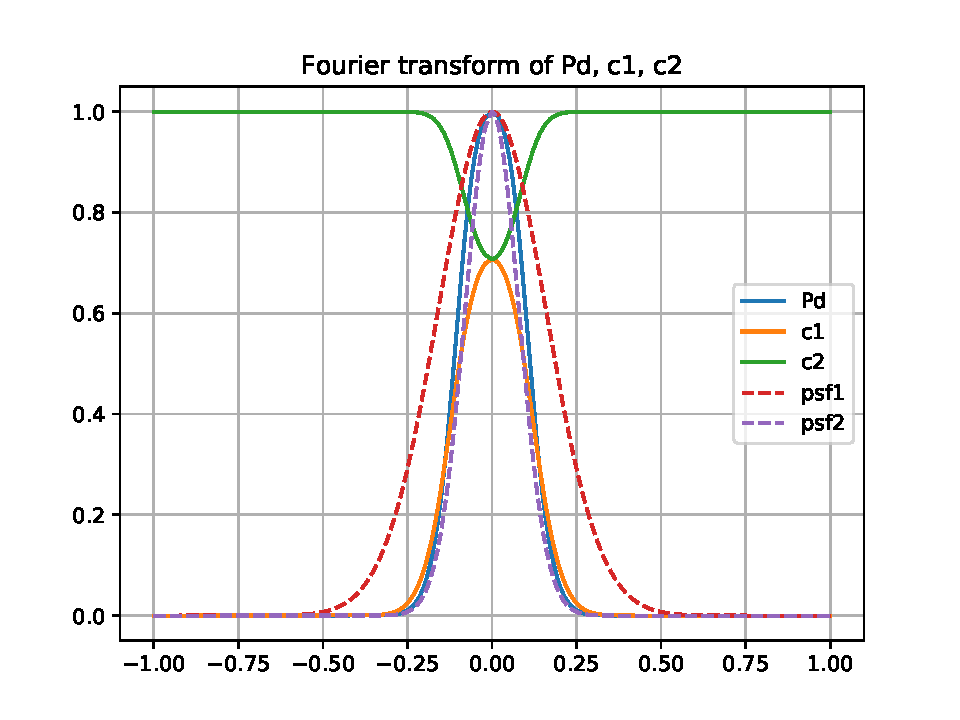
\includegraphics[width=5.5in]{fig/zogy_theo_Gaussians_ft_Pd_c1_c2.pdf}
\end{center}
\caption{\label{fig:theo_Gaussians_ft}1D slice along the x-axis in frequency
  space of the matching kernels and the PSF of the ZOGY difference
  image. The Fourier space representation of the input PSFs is also
  shown. The two PSFs have widths of $\sigma_1 = 1$, $\sigma_2 = 2$ in image
  space, i.e.\ \(\mathrm{PSF}_1\) is originally the narrower but the Fourier
  transformation swaps this relation.}
\end{figure}
%
\par In \Cref{fig:theo_Gaussians_ft}, we show 1D slices of the 2D solutions
of \(P_d\), \(c_1\) and \(c_2\). Noise variances and photometric scaling
factors are unity for simplicity. As the input PSFs are pure Gaussians,
i.e.\ symmetric, real value functions, their Fourier transforms are also
real and symmetric.\footnote{Detailed calculation notebooks are part of
  DM-26087.} Note the different behavior of the two matching kernels towards
high frequencies. The matching kernel of the narrower PSF image \(c_1\) goes
to zero, while the other one goes to unity here. While the graphs of \(c_1\)
and \(c_2\) resemble to Gaussians, they are not anymore, and we must use
numerical integration to calculate their inverse Fourier transform. Their
image space values for points along the x-axis is shown in
\Cref{fig:theo_Gaussians_img_c1,fig:theo_Gaussians_img_c2}.
%
\begin{figure}
\begin{center}
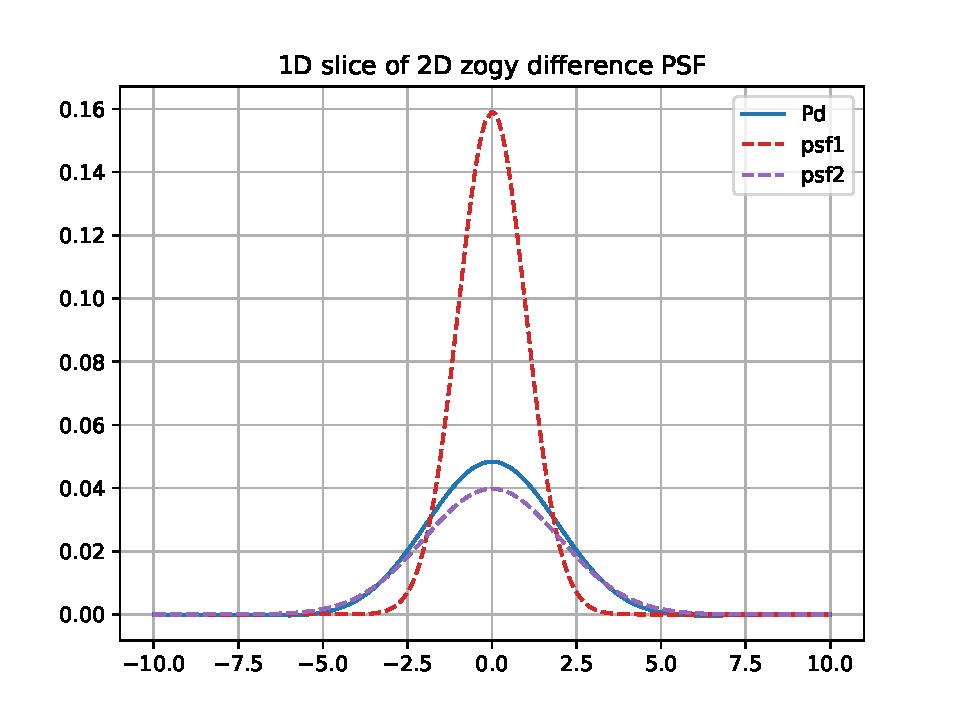
\includegraphics[width=5.5in]{fig/zogy_theo_Gaussians_img_Pd.pdf}
\end{center}
\caption{\label{fig:theo_Gaussians_img_Pd}1D slice along the x-axis in image
  space of the PSF of the ZOGY difference image with the input image PSFs.}
\end{figure}
%
\par In \Cref{fig:theo_Gaussians_img_Pd}, the PSF of the ZOGY difference
  image is shown. It is close to the wider input PSF, but strictly it's not
  a Gaussian, it has a negative overshoot, about 1\% of its peak
  value. This means that in an ideal case, signals in a ZOGY difference
  image are expected to have small negative rings around their positive
  peaks.
%
\begin{figure}
\begin{center}
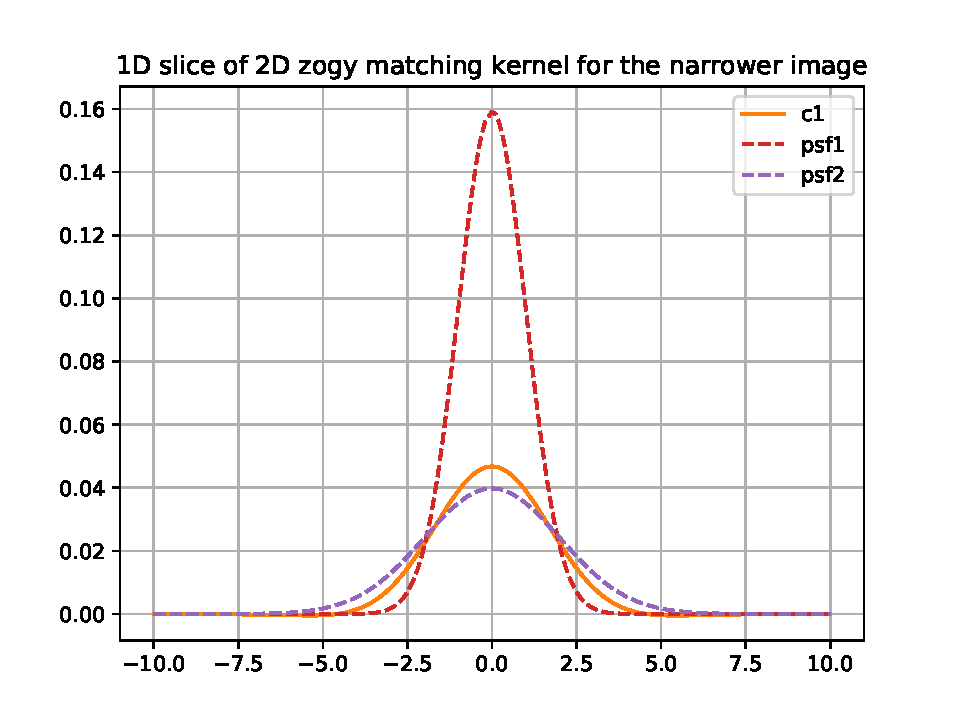
\includegraphics[width=4.5in]{fig/zogy_theo_Gaussians_img_c1.pdf}
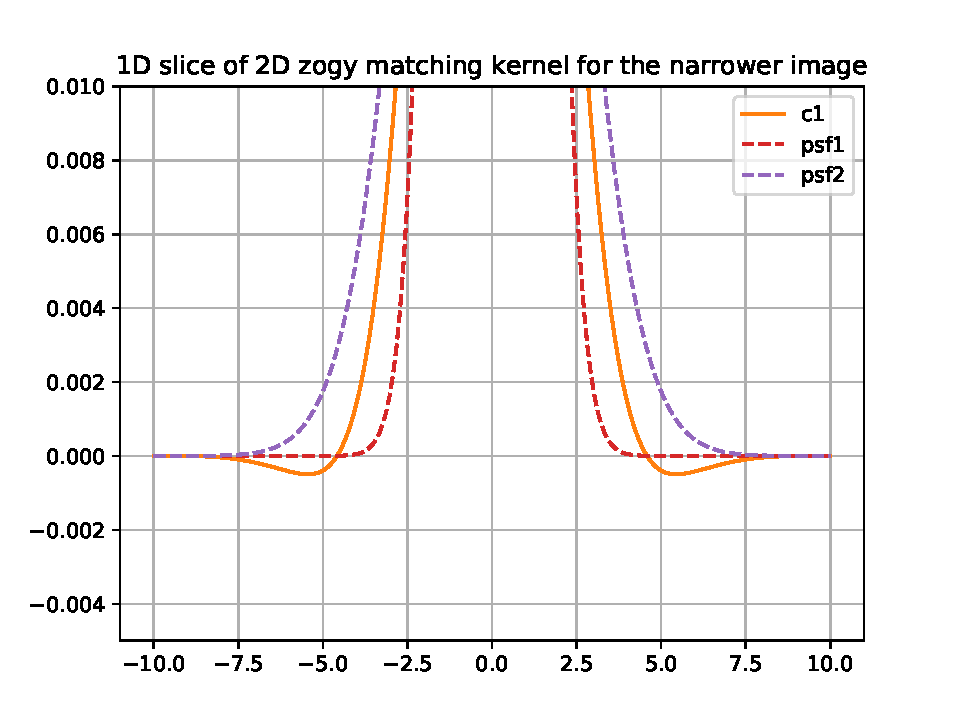
\includegraphics[width=4.5in]{fig/zogy_theo_Gaussians_img_c1_tails.pdf}
\end{center}
\caption{\label{fig:theo_Gaussians_img_c1}1D slice along the x-axis in image
  space of the matching kernel for the narrower PSF image. The matching
  kernel is a Gaussian-like curve that has a small oscillating correction in
  the tails.}
\end{figure}
%
\par For the narrower PSF input image, the matched PSF is created by
convolution with the matching kernel \(c_1\), shown in
\Cref{fig:theo_Gaussians_img_c1}. This matching kernel is similar to usual
Gaussian blurring but slightly narrower and has a negative tail itself.
%
\begin{figure}
\begin{center}
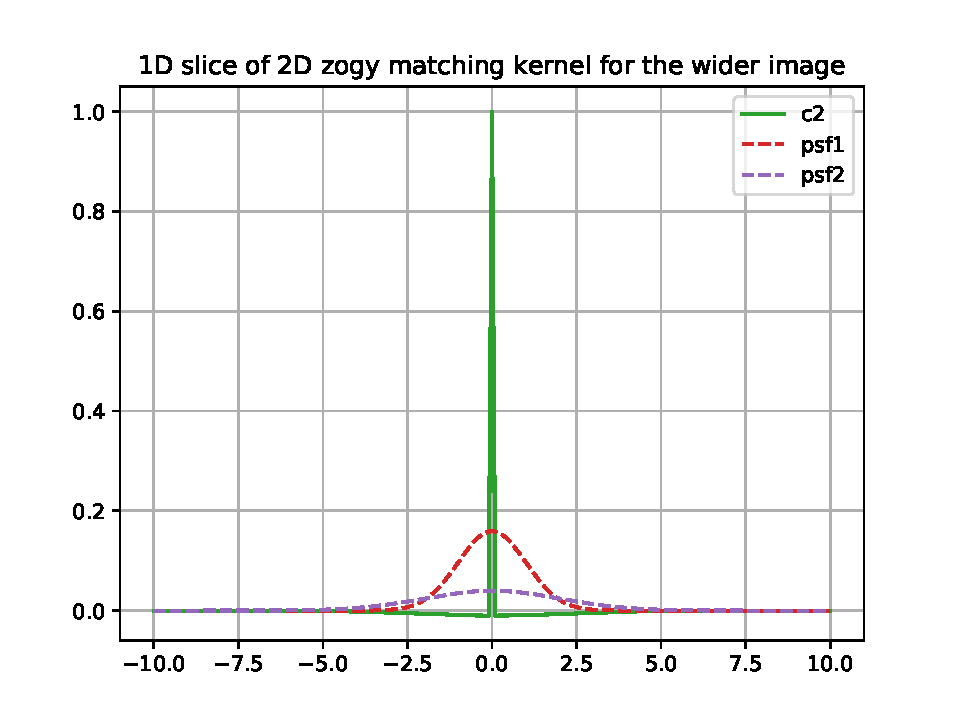
\includegraphics[width=4.5in]{fig/zogy_theo_Gaussians_img_c2.pdf}\,
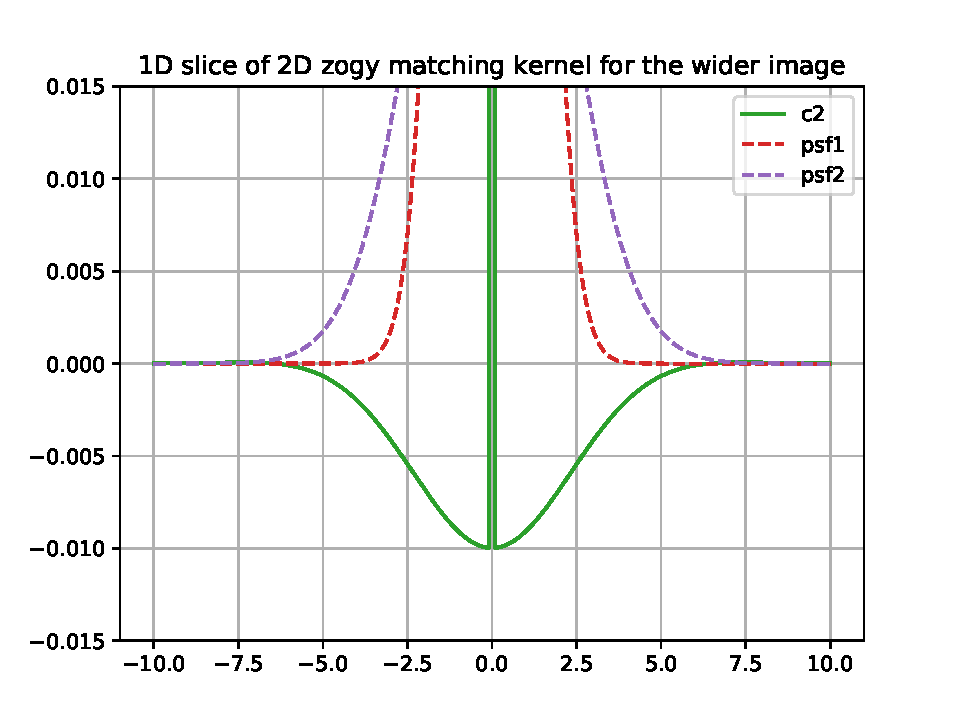
\includegraphics[width=4.5in]{fig/zogy_theo_Gaussians_img_c2_tails.pdf}
\end{center}
\caption{\label{fig:theo_Gaussians_img_c2}1D slice along the x-axis in image
  space of the matching kernel for the wider PSF image. The matching kernel
 is the sum of a Dirac delta minus a Gaussian-like curve.}
\end{figure}
%
\par For the wider image, the matching kernel \(c_2\) is an identity Dirac
delta kernel minus a Gaussian-like correction
(\Cref{fig:theo_Gaussians_img_c2}). The Dirac delta is the inverse transform
of the non-zero constant level of \(c_2\) in \Cref{fig:theo_Gaussians_ft}
that must be subtracted for the numerical integration to converge. The Dirac
delta peak is manually added to the result in \Cref{fig:theo_Gaussians_img_c2}.
%
\par Note that in case of identical PSFs, both \(c_1\) and \(c_2\) become
constant in \Cref{fig:theo_Gaussians_ft} which correspond to Dirac deltas in
image space. I.e. the matching operation is naturally reduced to the
identity operation if the two PSFs are already identical.
%
\clearpage
%
\section{The FFT calculated matching kernel of the ZOGY difference image\label{sec:ZOGYFFT}}
%
\par In practice, the ZOGY subtraction is implemented by Fast Fourier
Transforms (FFT). In this and the following sections, we study
practical numerical aspects of this approach.
%
\par In \Cref{fig:hits_zogy_artifacts}, we show typical patterns that appear
around features that do not subtract well. These sources are present in all
visits in the HiTS2015 data AL image difference processings and in some
visits they produce different artifacts in the AL subtraction as well;
however, AL artifacts are spatially more localized to the source than in the
ZOGY case. The ZOGY patterns can also appear in the vicinity of masked
regions, cosmic rays, or close to the image edges.
%
\begin{figure}
\begin{center}
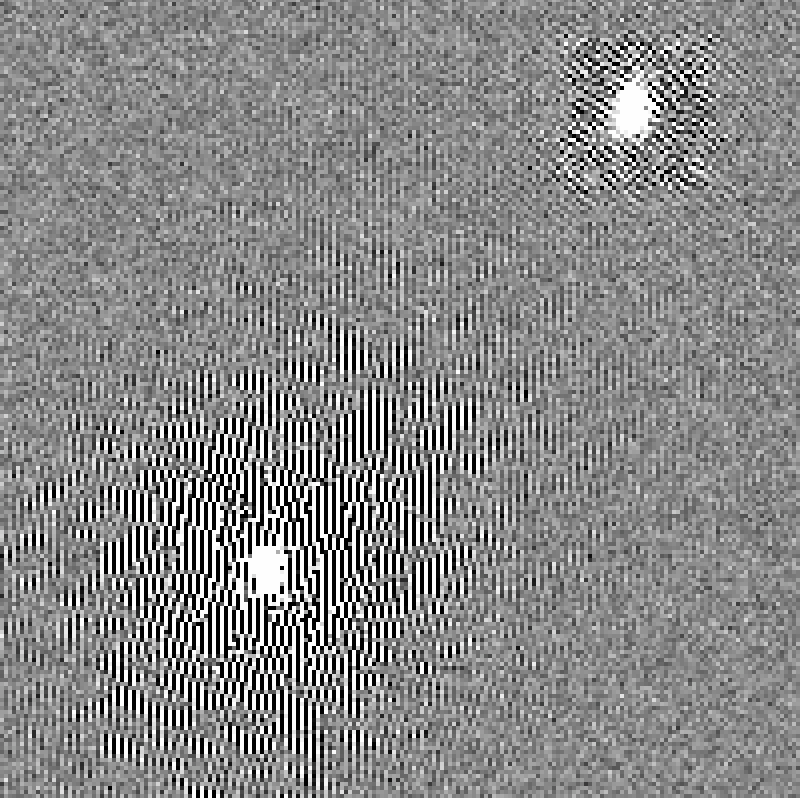
\includegraphics[width=3in]{fig/zogy_artifacts_v412060.png}
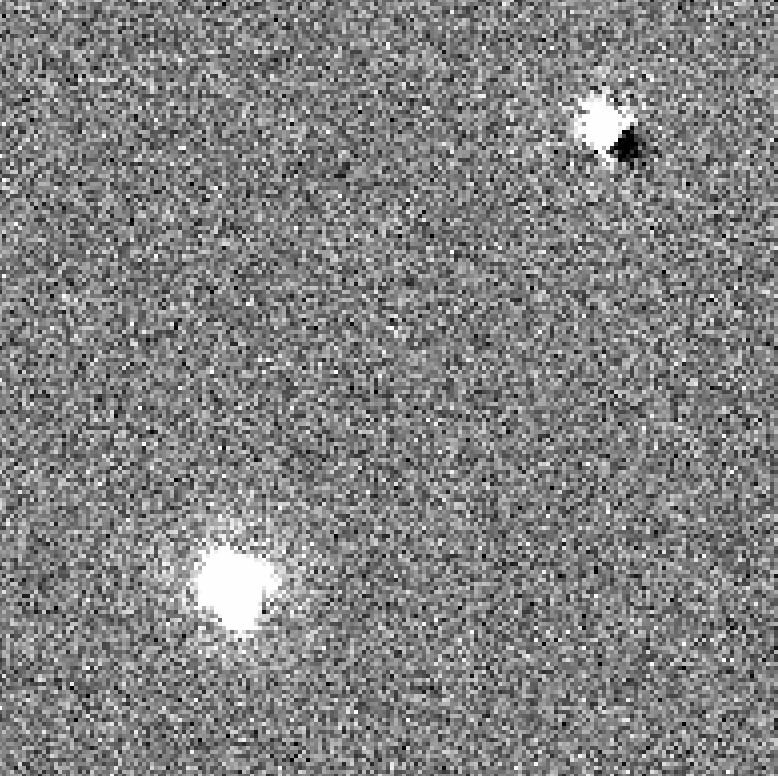
\includegraphics[width=3in]{fig/AL_goodvisit_v412060.png}
\end{center}
\caption{\label{fig:hits_zogy_artifacts}High frequency artifacts in the ZOGY
  difference image (left) around bright sources that are present in all
  visits in the AL processing as well. In the same visit, the AL subtraction
  (right) has less pronounced visual imperfections.}
\end{figure}
%
\subsection{Zero values of the PSF\label{sec:PSFzero}}
%
\par In \Cref{eq:Dhat}, \(\hat{D}\) is not defined at frequencies where both
image PSFs are zero. Indeed, according to the image models (\Cref{eq:N}), at
these frequencies, the input images do not carry any information about the
true image. They consist of pure noise. In accordance with this, these
frequencies have zero contribution to \(\hat{S}\).
%
\par We cannot allow zero division in our calculations anyway, thus we
need to have a workaround for pixels where the denominator in
\Cref{eq:S,eq:Dhat} are zero. We define \(\hat{D}\) at these
frequencies as the straightforward subtraction of the two images with
the same scaling to keep the variance constant at all
frequencies. Of course, \(\hat{S}=0\) at these pixels. This is
currently implemented in the code stack.
%
\subsection{Matching kernel limit values in frequency space\label{sec:FFTlimits}}
\begin{figure}
\begin{center}
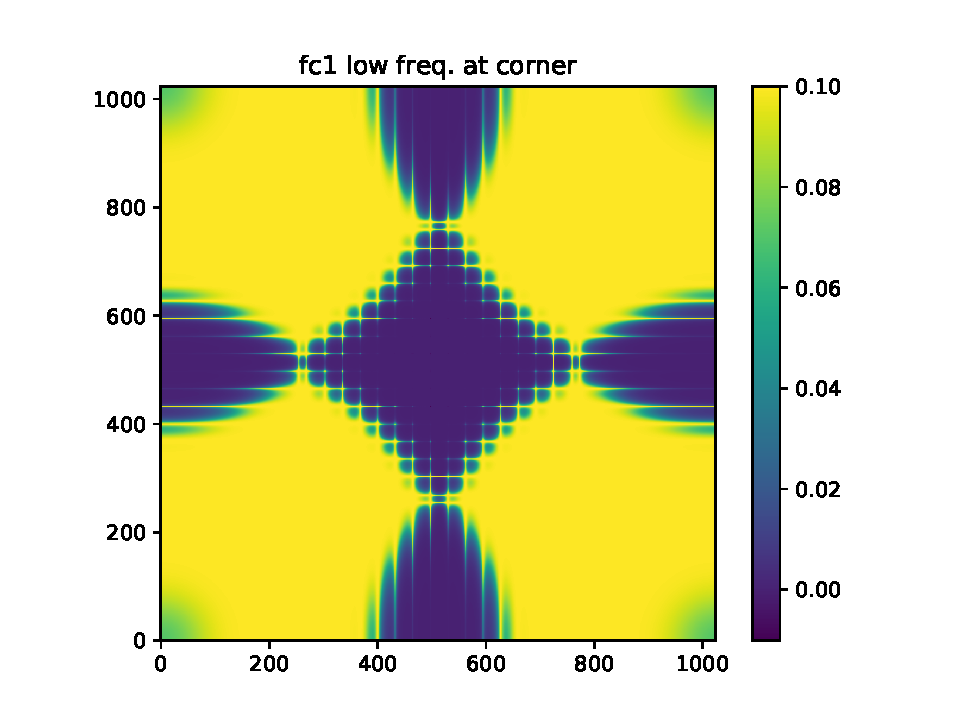
\includegraphics[width=5.5in]{fig/fft_steps_fc1.pdf}
\end{center}
\caption{\label{fig:fft_steps_fc1}FFT calculated matching kernel for two
  Gaussian PSFs, here for the wider PSF image. This is a Fourier space image
  with low frequencies at the corners. In this calculation \(\sigma_1=3.3\),
  \(\sigma_2=2.2\) PSFs were generated in a 31x31 size image, that were zero
  padded to 1024x1024 image size before FFT. Per pixel noise variance is 100
  for both images, photometric scalings are unity. All values are real due
  to symmetry in the inputs.}
\end{figure}
%
\begin{figure}
\begin{center}
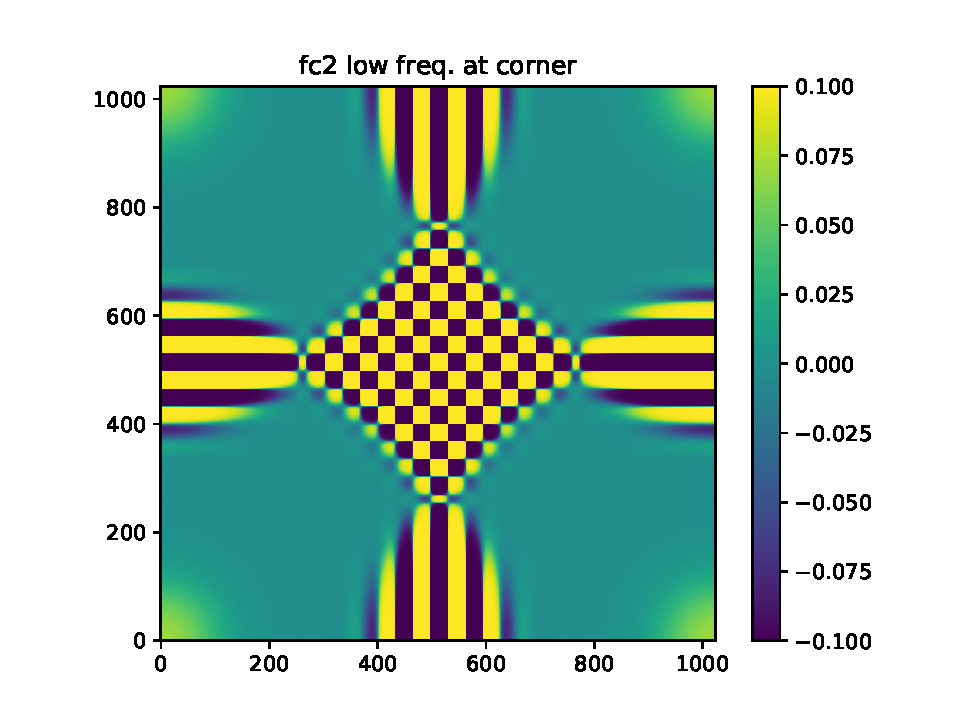
\includegraphics[width=5.5in]{fig/fft_steps_fc2.pdf}
\end{center}
\caption{\label{fig:fft_steps_fc2}FFT calculated matching kernel for the
  narrower PSF image. This is a Fourier space image with low frequencies at
  the corners. All values are real due to symmetry in the inputs.}
\end{figure}
%
\par We saw in the theoretical solution section, that in case of
Gaussian PSF-s, the matching kernels in frequency space have tails
converging to different limit values. The limit values are either zero
or a non-zero constant depending on whether the matching kernel belongs
to the narrower or wider input PSF image, respectively.
%
\par In \Cref{fig:fft_steps_fc1,fig:fft_steps_fc2}, \(\hat{c}_1\),
\(\hat{c}_2\) are calculated from two 31x31 pixel size Gaussian PSFs
that were zero padded for a 1024x1024 image size, with
\(\sigma_1=3.3\), \(\sigma_2=2.2\).\footnote{Detailed calculation
notebooks are part of DM-26941.} All numbers are real in this
case. The shown frequency space images are in their natural FFT
orientation with zero frequencies at the corners and highest
frequencies in the centers. Starting from the corners, both solutions
follow our expectations, converging either down to zero or to their
expected non zero constant (\( 1/\sigma_{\mathrm{pixelnoise}} \) )
plateau. The trend breaks for both kernels in high frequency regions
however, and high value noise appears.
\begin{equation}
\hat{c}_1 \sim \frac{1}{\sqrt{1 + \left(\frac{\hat{P}_1}{\hat{P}_2}\right)^2}}
\label{eq:c1conv}
\end{equation}
\par The matching kernel limit values depend on whether
\(\hat{P}_1/\hat{P}_2\) is converging to zero or diverges as it can be seen
in \Cref{eq:c1conv}. Once we reach the point where the Gaussian tails are
dominated by noises\footnote{See \Cref{sec:floating_point}}, the convergence
properties of these fractions become lost and the calculated matching kernel
values significantly deviates from their expected limit values.
%
\subsection{Patterns in image space\label{sec:patterns}}
\par What does this mean for our calculated matching kernels back in
image space?
%
\par In \Cref{fig:twoG_c1}, we show \(c_1\) transformed and
re-centered back to image space (but still in its fully padded image
size). The purple structure indicates that there is a sign oscillation
pattern all accross padded size image.
\begin{figure}
\begin{center}
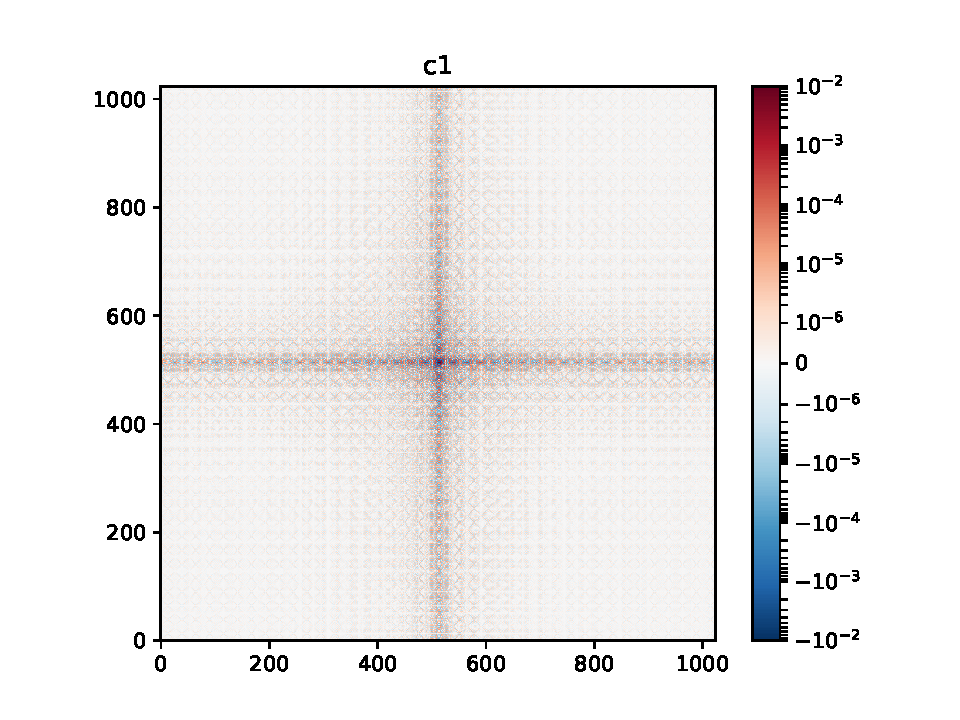
\includegraphics[width=5.5in]{fig/twoG_defaults_c1.pdf}
\end{center}
\caption{\label{fig:twoG_c1}Two Gaussian PSFs with spatial widths of \(\sigma_N = 3.3\)
  \(\sigma_R = 2.2\) pixels. \(c_1\), the ZOGY matching convolution in image space
  of the new (\(N\)) image. The purple pattern is an indication of
  sign oscillation all over the image.}
\end{figure}
%
\par We can see that in the direction of the two axes, there are definite
purplish patterns. The purple color on this red-blue color scale shows a
sign oscillation that can be verified in zoomed-in versions of the
figure. These patterns do not fade away in the direction of the axes from
the center, indicating that these oscillating sign values have roughly the
same order of magnitude absolute values. The original PSF size 31x31 cannot
be clearly identified any more in the image either. We note that
the appearance of these patterns is independent of the padding
size.
%
In \Cref{fig:twoG_pd} \(P_d\) is shown, calculated by \Cref{eq:Pdhat}.
\begin{figure}
\begin{center}
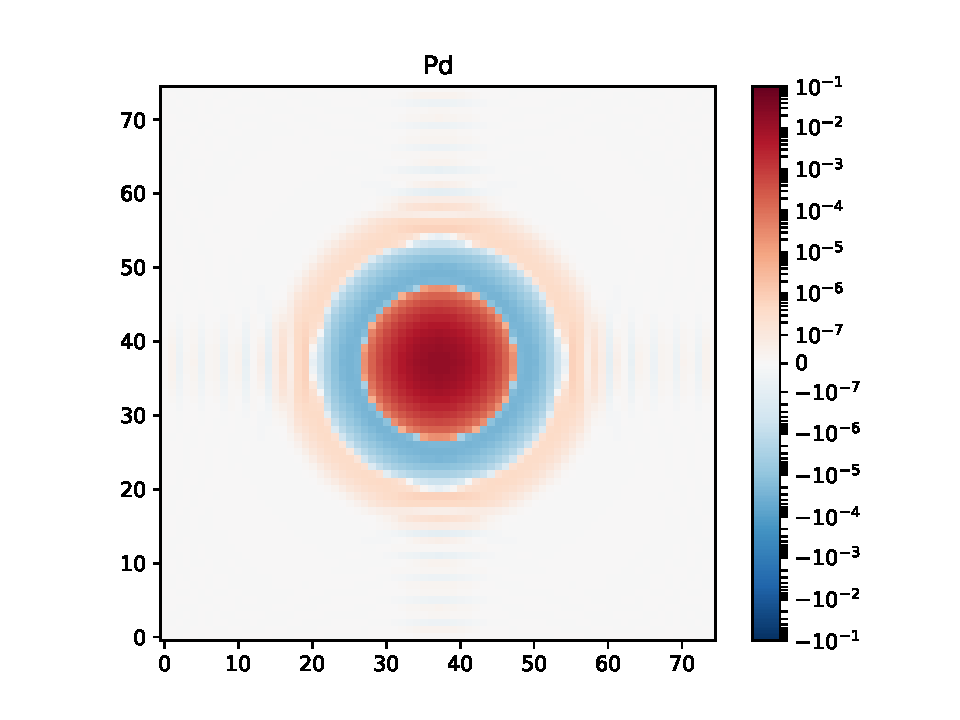
\includegraphics[width=5.5in]{fig/twoG_defaults_Pd.pdf}
\end{center}
\caption{\label{fig:twoG_pd}Two Gaussian PSFs with spatial widths of
  \(\sigma_N = 3.3\) \(\sigma_R = 2.2\). \(P_d\), the PSF of the zogy
  difference image.}
\end{figure}
We also show the PSF of \(S\) in \Cref{fig:twoG_ps}. The PSF of the
score image shows how a Dirac delta signal (in the truth image)
appears in \(S\), though in source detection, only the actual pixel
values matter in \(S\), the shape of the PSF does not.
\begin{figure}
  \begin{center}
    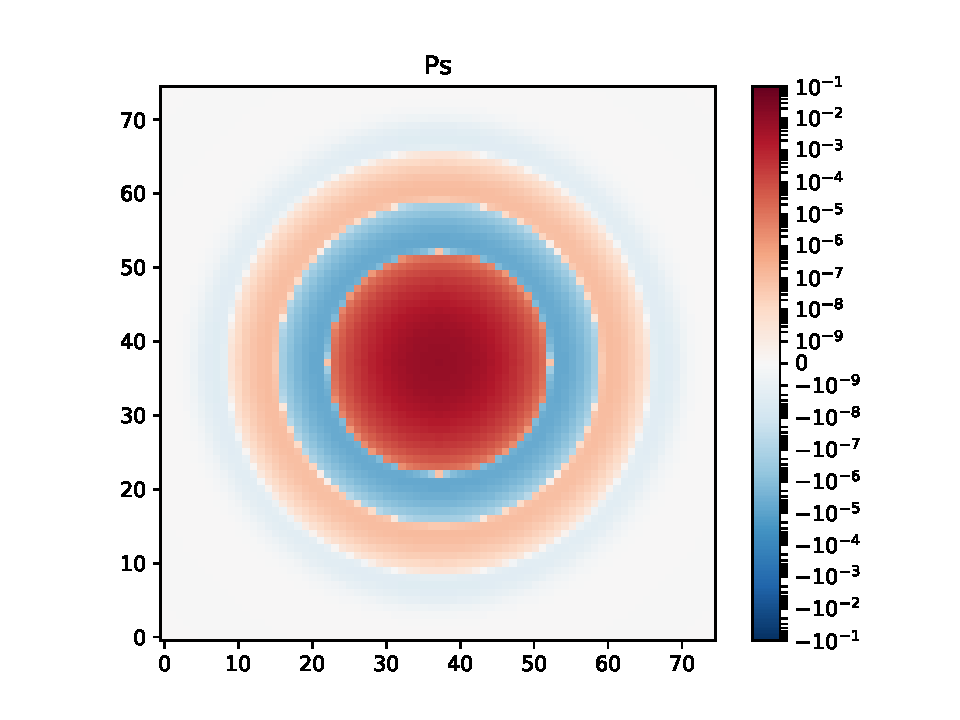
\includegraphics[width=5.5in]{fig/twoG_defaults_Ps.pdf}
  \end{center}
\caption{\label{fig:twoG_ps}Two Gaussian PSFs with spatial widths of
  \(\sigma_N = 3.3\) \(\sigma_R = 2.2\) \(P_s\), the PSF of the score
  image.}
\end{figure}
%
\par \(P_d\) and \(P_s\) have much cleaner images, contained in size
in image space, and close to our theoretical
expectations. (\(\hat{P}_s \sim \hat{P}_d \overline{\hat{P}_d}\)).
%
\par Recall that while we expressed \(P_d\) in \Cref{eq:Pdhat} as the
function of the input PSFs, in a difference image this is the result
of the convolution of the images with the matching kernels.  The high
frequency noise in the matching kernel is not disturbing, so long the
image follows the model PSF assumption and has approximately Gaussian
PSF features that suppress high frequencies. If there are edges, or
signals with high frequency components in the input images, the noisy
high frequency features of the matching kernel becomes visible in the
difference image. Our current understanding is that the deviation of
the image PSF from the model assumption and the numerical noise
in the matching kernels together cause the visible artifacts in the
difference images produced by the code stack. This conclusion is
supported by tests on simulated images that have sources only with
perfect Gaussian PSFs. In these cases, no visual artifacts can be seen.
%
\subsection{Workaround for artifact suppression\label{sec:workaround}}
We propose the following workarounds for the difference image artifact
problem:
\begin{itemize}
  \item In a Gaussian PSF approximation, we can directly create the
    PSF in the padded, full-size frequency space, avoiding the zero
    padding of a small image then the FFT operation. However, this
    approach restricts our input kernels strictly to Gaussians.
  \item In a more generic approach, we can still use the padded, FFT-d
    detected PSFs of the input images. Using a radius approximation, we
    can determine which input PSF is the wider one in a Gaussian
    approximation. Then we can introduce a configurable threshold in
    \emph{frequency space} and pixels in the matching kernels can be
    replaced with their Gaussian limit values wherever the input PSFs
    go below the threshold (in absolute value, in frequency space).
  \item As a third option, we should recall, that the noise artifacts
    appear only in the difference image. In the score image, these are
    automatically suppressed by further convolution with \(P_d\). We
    can choose to use the score image only directly for detection
    significance.
\end{itemize}
%
\par We repeated the above exercise by generating the Gaussian PSFs directly
in frequency space and performed exactly the same matching kernel and
\(P_d\) calculations. These results can be seen in
\Cref{fig:fft_steps_direct_fc1fc2,fig:fft_steps_direct_c1c2,fig:fft_steps_direct_Pd}. These
solutions fully satisfy the theoretical limit values and their image space
counterparts are free from any noisy patterns.
%
\begin{figure}
\begin{center}
  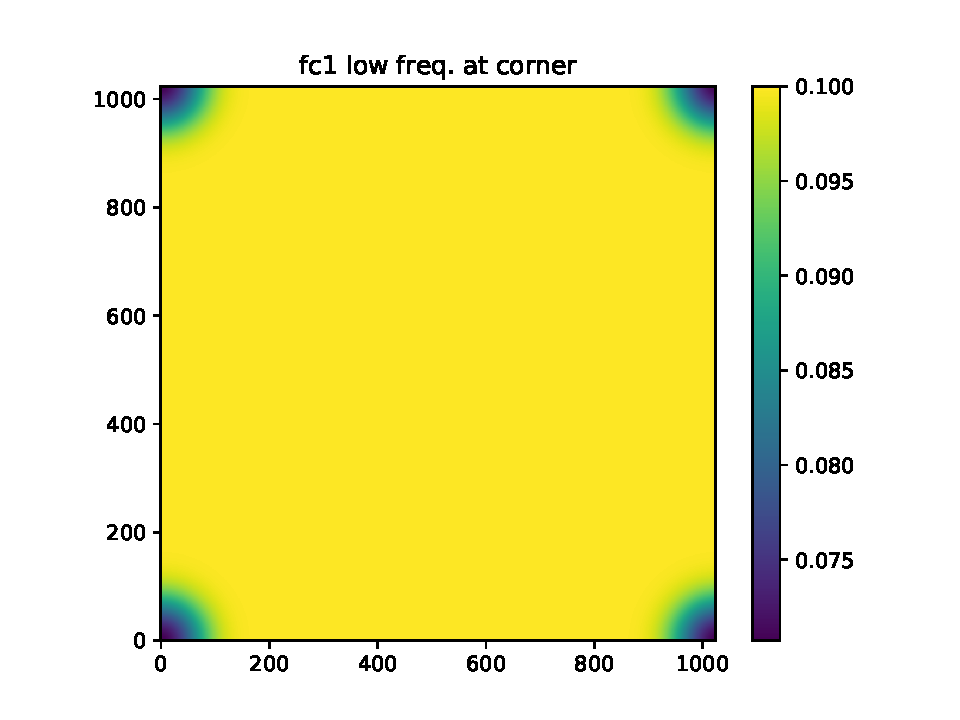
\includegraphics[width=4.5in]{fig/fft_steps_direct_fc1.pdf}
  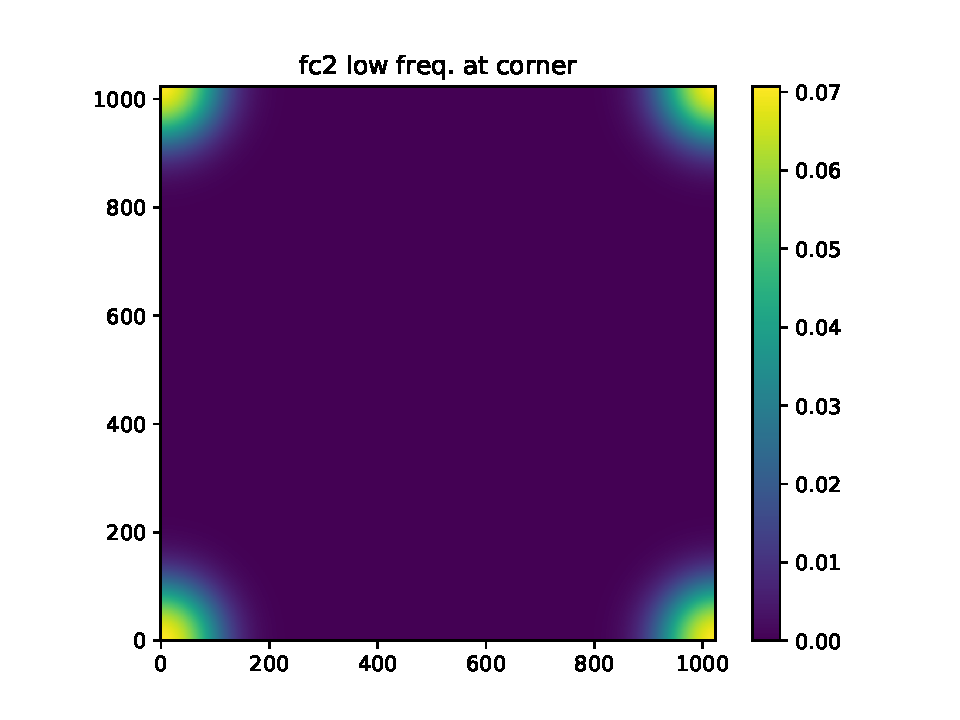
\includegraphics[width=4.5in]{fig/fft_steps_direct_fc2.pdf}
\end{center}
\caption{\label{fig:fft_steps_direct_fc1fc2}The matching kernels for two
  Gaussian PSFs in frequency space. In this calculation, PSFs were
  directly generated in an 1024x1024 frequency space image
  corresponding to image space \(\sigma_1=3.3\), \(\sigma_2=2.2\)
  widths. Per pixel noise variance is 100 for both images, photometric
  scalings are unity.}
\end{figure}
%
\begin{figure}
\begin{center}
  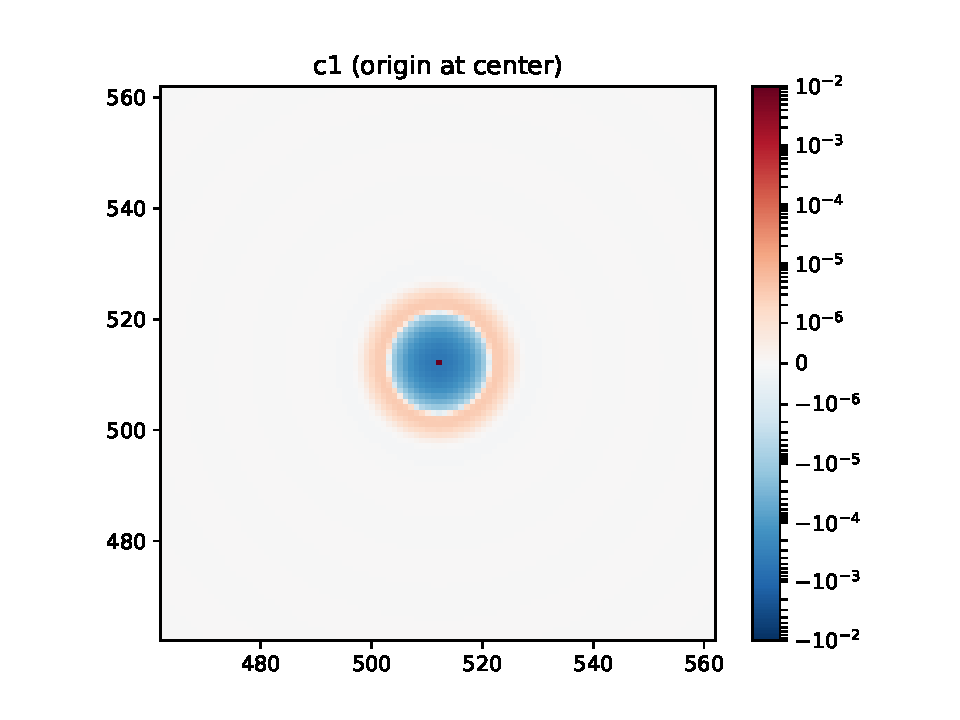
\includegraphics[width=4.5in]{fig/fft_steps_direct_c1_zoomed.pdf}
  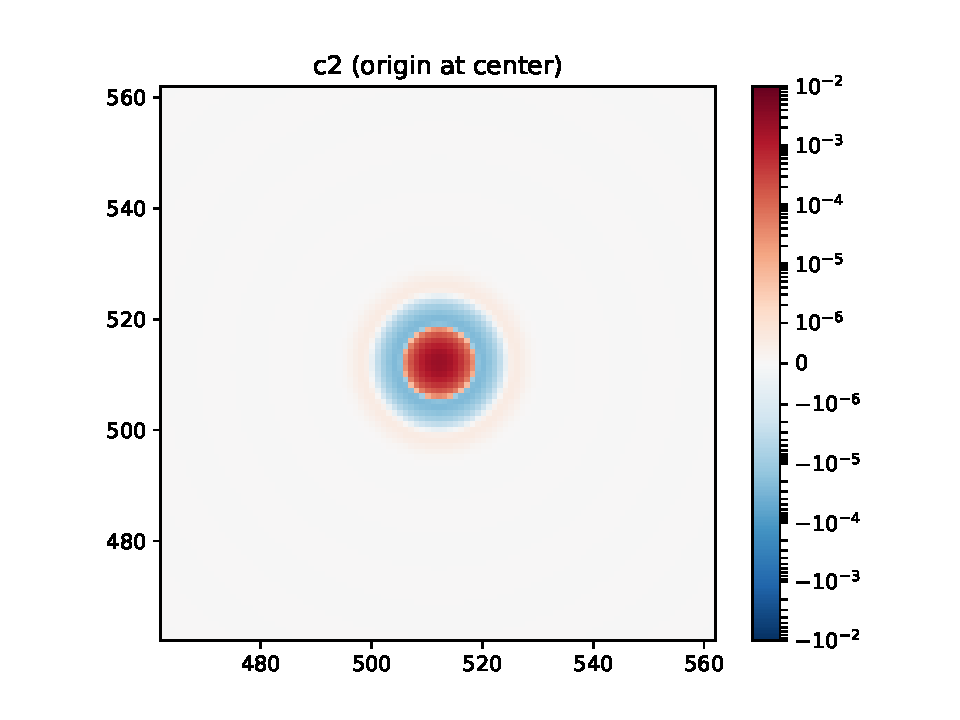
\includegraphics[width=4.5in]{fig/fft_steps_direct_c2_zoomed.pdf}
\end{center}
\caption{\label{fig:fft_steps_direct_c1c2}The matching kernels inverse
  FFT-d into image space, re-centered and zoomed in for
  details.}
\end{figure}
%
\begin{figure}
\begin{center}
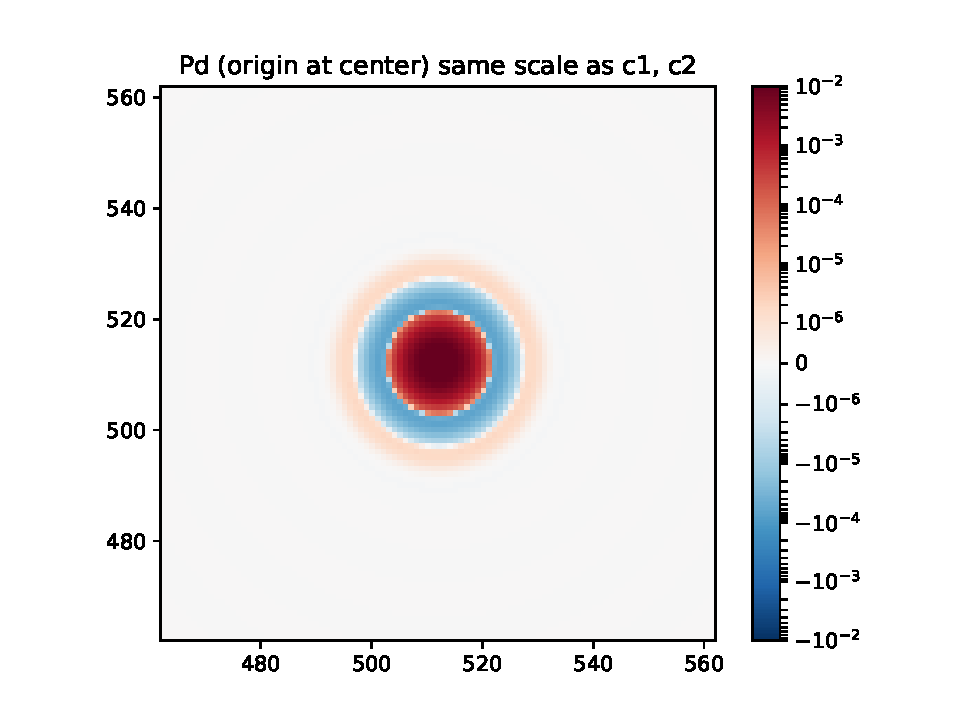
\includegraphics[width=5.5in]{fig/fft_steps_direct_Pd_zoomed.pdf}
\end{center}
\caption{\label{fig:fft_steps_direct_Pd}The difference image PSF
  inverse FFT-d into image space, re-centered and zoomed in for
  details.}
\end{figure}
%
\clearpage
%
\section{Variance plane calculation of the difference image\label{sec:varplane}}
\par While the ZOGY image model does not strictly allow for different
per-pixel noise values (its noise model assumes homogeneous variance
noise across all pixels), from the \Cref{eq:c1N_c2R} form of the
difference image, we can propagate the different pixel variance
information in the variance planes into the difference image. To do
this, we notice that if we do convolution on an image of independent
noise then, in image space, the variance plane should be convolved by
the square of the convolution kernel. This is the well-known square
addition of variances of independent random variables.\footnote{See
  also ZOGY paper eqs. 26-29.}
%
\par We'd like to emphasize that this step cannot be applied to an
image with already correlated noise; the square addition of pixel
noise in the variance plane do not account for the covariance terms
and would result in underestimation of the pixel
variance. Notably, the effect of a noise decorrelation
(whitening) kernel on an already convolved image cannot be applied to
the variance plane based on the square addition rule as it would lower
the variance further instead of reverting it to the uncorrelated
level. In accordance with this, the image space square operation is
not distributive with respect to convolution in general; the square of the
convolution of two kernels is not the same as the convolution of the
squared kernels, and we should always perform the former.
%
\par To calculate the variance plane of the difference image, we
should calculate \(c_n\), \(c_r\) in \Cref{eq:c1N_c2R}, transform them
back to image space, square them in image space, and convolve the
original images' variance planes with these squared matching
kernels. In practice, this convolution is more straightforward to be
performed in frequency space again because these images already share
common, full image size dimensions (the dimensions of our ZOGY
frequency space calculations).
%
\par \Cref{eq:Shat} can also be written similarly to \Cref{eq:c1N_c2R} and
the variance plane of S can be calculated this way as well.
%
\section{ZOGY and AL equivalence\label{sec:ALZOGYequiv}}
%
\par In \Cref{eq:DzPz}, we write the ZOGY score image in frequency
space and expand the expression to demonstrate that the AL matching
and subtraction combined with the decorrelation afterburner noise
whitening theoretically leads to the same detection statistics.  In the
AL case the role of the two images are not symmetric, the template PSF
is matched to the science image, and the science image is left
intact. Assuming that the AL optimization finds the perfect matching
kernel, it should be \(P_n/P_r\).  Indeed, considering the score
image, the difference between the AL and ZOGY images are only a factor
of \(\hat{P}_r/\abs{\hat{P}_r}\). Compared to the AL, in the ZOGY case
both the difference image and its PSF carry an extra
\(\hat{P}_{pre}/\abs{\hat{P}_{pre}}\) factor that cancel from the
overall expression of the score image. Indeed, as
\(\overline{\hat{P}_r}\hat{P}_r/\abs{\hat{P}_r}^2 = 1\), this factor
can be arbitrarily added to or removed from the difference image
and PSF terms without changing the resulting score image.
%
\par Furthermore, note that \(\hat{P}_r\) from the AL perspective can
be treated as an optional \emph{pre-convolution} kernel for the
science image. If we use the decorrelation afterburner with the
correction term that includes the pre-convolution kernel
(\Cref{eq:KPre,eq:DalPre}), the AL approach with the decorrelation
afterburner will still lead to the same score image.
%
\par If we select the PSF of the \emph{template} as pre-convolution
kernel for the science image, the AL difference image solution should
be exactly the same as the ZOGY proper difference image. However, we
can use \emph{any} pre-convolution kernel. We think that the real
question is what pre-convolution kernel should be used so that the AL
algorithm has a good quality stable performance in finding the
matching kernel solution. The performance may vary as the matching
kernel solution includes the pre-convolution kernel, and the
pre-convolved science image does not have uncorrelated noise during
the AL numerical optimization. Strictly speaking, correlated noise
violates the optimization algorithm’s noise assumptions, but we don't think this is a
major factor in its performance in practice. This could be studied in the future.
%
\begin{equation}
F_D = \frac{1}{\sqrt{\frac{\sigma_n^2}{F_n^2} + \frac{\sigma_r^2}{F_r^2}}}
\end{equation}
%
\begin{align}
  \hat{S} \sim \hat{D}_Z\overline{\hat{P}_Z} &= \frac
  {\frac{\hat{P}_r\hat{N}}{F_n} - \frac{\hat{P}_n\hat{R}}{F_r}}
  {\sqrt{\frac{\sigma_n^2}{F_n^2}\abs{\hat{P}_r}^2 +
      \frac{\sigma_r^2}{F_r^2}\abs{\hat{P}_n}^2}}
  \cdot
  \frac{\overline{\hat{P}_n\hat{P}_r}\sqrt{\frac{\sigma_n^2}{F_n^2} + \frac{\sigma_r^2}{F_r^2}}}
  {\sqrt{\frac{\sigma_n^2}{F_n^2}\abs{\hat{P}_r}^2 +
      \frac{\sigma_r^2}{F_r^2}\abs{\hat{P}_n}^2}} = \label{eq:DzPz}\\
 &= F_D \frac
  {\left(\frac{\hat{N}}{F_n} -  \frac{\hat{R}}{F_r} \cdot
    \frac{\hat{P}_n}{\hat{P}_r}\right) \sqrt{\frac{\sigma_n^2}{F_n^2} + \frac{\sigma_r^2}{F_r^2}} }
  {\sqrt{\frac{\sigma_n^2}{F_n^2} +
      \frac{\sigma_r^2}{F_r^2}\abs{\frac{\hat{P}_n}{\hat{P}_r}}^2}}
  \cdot
  \frac{\hat{P}_r}{\abs{\hat{P}_r}}
  \cdot
  \frac{\overline{\hat{P}_n\hat{P}_r}\sqrt{\frac{\sigma_n^2}{F_n^2} + \frac{\sigma_r^2}{F_r^2}}}
  {\sqrt{\frac{\sigma_n^2}{F_n^2}\abs{\hat{P}_r}^2 +
      \frac{\sigma_r^2}{F_r^2}\abs{\hat{P}_n}^2}} = \\
  &= F_D \hat{D}_{AL} \cdot \frac{\overline{\hat{P}_n}
  \sqrt{\frac{\sigma_n^2}{F_n^2} + \frac{\sigma_r^2}{F_r^2}}}
  {\sqrt{\frac{\sigma_n^2}{F_n^2} +
      \frac{\sigma_r^2}{F_r^2}\abs{\frac{\hat{P}_n}{\hat{P}_r}}^2}} =
F_D \hat{D}_{AL}\overline{\hat{P}_{AL}}
\label{eq:DalDzPrPr}
\end{align}
%
\begin{equation}
\hat{D}_{AL} = \frac{\hat{D}_Z}{F_D}\cdot\frac{\abs{\hat{P}_r}}{\hat{P}_r}
\end{equation}
%
\begin{align}
  \hat{D}_{AL} &= \frac
  {\frac{\hat{P}_{pre}\hat{N}}{F_n} -
    \frac{\hat{P}_n\hat{P}_{pre}\hat{R}}{\hat{P}_r F_r} }
  {\sqrt{\frac{\sigma_n^2}{F_n^2}\abs{\hat{P}_{pre}}^2 +
      \frac{\sigma_r^2}{F_r^2}\abs{\frac{\hat{P}_n\hat{P}_{pre}}{\hat{P}_r}}^2}}
  \sqrt{\frac{\sigma_n^2}{F_n^2} + \frac{\sigma_r^2}{F_r^2}}
                 \label{eq:DalPre}
\end{align}
%
\section{Decorrelation afterburner normalization}
\par To preserve the photometric scale of the AL difference
image (that is the same of the science image), the decorrelation
afterburner correction should be overall a convolution with a
normalized correction kernel (in image space). PSF normalization can
be easily ensured in frequency space. If we evaluate any PSF at 0,
based on \Cref{eq:X0sum} they should give 1. The AL matching kernel is
not constrained this way in general. The sum of the AL matching kernel
and the optional pre-convolution kernel can be written as separate
factors in the decorrelation afterburner. The correctly normalized
decorrelation afterburner is written in \Cref{eq:KPre}.\footnote{As of
  writing this is not implemented in the LSST stack correctly. It is
  DM-25050.}
%
\begin{align}
  \hat{K} &= \frac{\sqrt{\frac{\sigma_n^2}{F_n^2}S_{pre}^2 + \frac{\sigma_r^2}{F_r^2}S_{mk}^2}}
  {\sqrt{\frac{\sigma_n^2}{F_n^2}S_{pre}^2\abs{\hat{P}_{pre}}^2 + \frac{\sigma_r^2}{F_r^2}S_{mk}^2
  \abs{\hat{P}_{mk}}^2}}
\label{eq:KPre}
\end{align}
%
\section{Conclusions}
%
\par We studied the ZOGY difference image matching kernels for Gaussian
input PSFs in this document. In the thoretical calculations
(\Cref{sec:ZOGYtheo}), we showed that the matching kernels have different
convergence values in their tails depending whether they belong to the
narrower of wider PSF input image. In practice, using FFT, these convergence
properties are not well reproduced and the resulting image space matching
kernels have oscillating patterns all over the image
(\Cref{sec:ZOGYFFT}). We concluded that this noise is still acceptable if
the input images follow their PSF models and suppress high frequencies,
however noise patterns appear in the difference image if the PSFs
deviate. This noise is extended, visually unappealing, and can disrupt other
algorithms' performance on the difference image; however, it has little
impact on the source detection statistic.
%
\par We tested the direct Gaussian PSF generation in frequency space as a
possible way to avoid the convergence problems in our calculations. We
expect that it would produce difference images without large scale patterns
for all inputs. It is a strong restriction on the PSFs, so we also plan to
look for weaker constraints in suppressing the artifacts in the difference
image. We also need to consider sampling (aliasing) details before
implementation.
%
\par In \Cref{sec:varplane} we discussed how to properly calculate the variance
plane in frequency space when we have noise whitening decorrelation
operations.
%
\par In \Cref{sec:ALZOGYequiv}, we demonstrated that the AL method combined with
the decorrelation afterburner leads to the same detection statistic as the
ZOGY method. With preconvolution, they can theoretically lead to the very
same difference image. We believe though that his approach would meet
similar practical problems as the ZOGY subtraction has. This is a possible
future topic to study.
%
\par In \Cref{sec:appendix} we discuss various considerations that have
relevance in the actual and for future frequency space image differencing
code implementations.
%
\par Finally, the noisy matching kernels cause complications in
implementing solutions in frequency space for spatial variations of the PSF
in a large image. This is also a topic we plan to study in the future.

